\label{desenvolvimento_estrutura}

A solução proposta para o módulo mecânico/estrutural está descrita nesta seção.

\subsection*{Seleção de materiais e faixas de atuação}

\subsubsection*{\textbf{Materiais para a estrutura da bancada}}

A base estrutural da mesa de vibração será composta por cantoneiras de abas iguais. A cantoneira a ser utilizada terá abas iguais e uma bitola de 4,76 x 50,8mm, tendo assim um peso de 3,63kg/m. Com esse peso, será atendido o objetivo da base da estrutura de ter um peso elevado afim de que as vibrações do motor não sejam transmitidas para a base da mesa. Tendo em vista que será utilizado 8,89 metros deste material para compor a estrutura da base, totalizando assim um peso de 32,27kg atendendo a perspectiva de uma base de peso elevado. 

Além do peso, a cantoneira de tal espessura de aço 1010 atende as especificações do projeto no que tange integridade estrutural, fazendo com que a base da mesa não sofra flexão, torção, dentre outros momentos estruturais que levam em conta a integridade da mesa \cite{acos_continente}.

Fazendo uma comparação com outros materiais verificou-se que a cantoneira é a geometria de material que melhor atende a fabricação da base estrutural da mesa. Um perfil retangular vazado fabricado de \textit{metalon} era uma boa opção, porém não atendia os objetivos de obtenção do peso elevado, e da boa integridade estrutural. Por se tratar de um aço estrutural de baixas propriedades mecânicas a possibilidade da mesa sofrer flexão ou torção seria aumentada. Com base nisso a escolha do material da base da estrutura estará satisfeita com a utilização de cantoneira do tipo abas iguais de aço 1010 com bitola de 4,76 x 50,8mm. 

	A bancada terá 4 molas fixadas nas extremidades da superfície vibratória e na estrutura da base. Essas molas serão usadas com intuito de amortecer e absorver a vibração da superfície vibratória para evitar a propagação vibracional e a força compressiva na estrutura, ao mesmo tempo, as molas auxiliarão na vibração da superfície superior da mesa \cite{mola_santos}.
    
	As molas que serão utilizadas terão a composição formada por dois batentes de borracha intermediários. Foram devidamente projetadas para garantir uma grande eficácia na eliminação das vibrações para a estrutura, sendo capazes de reduzir em até 95\% a propagação da vibração da superfície vibratória para a estrutura \cite{mola_catalogo}.
    
    A bancada terá 4 pés, de borracha e ferro, para que as vibrações fiquem mais distribuídas e não sobrecarreguem apenas uma aresta. Outro fator importante é que os 4 pés juntos suportam ate 100 kg, o que atende as exigências relacionadas a massa estipulada no projeto \cite{ferramentas_kennedy}.
    
    Um desenho técnico do pé da mesa é apresentado na Figura \ref{fig:pe_bancada}.
    
    \begin{figure}[!ht]
      \centering
      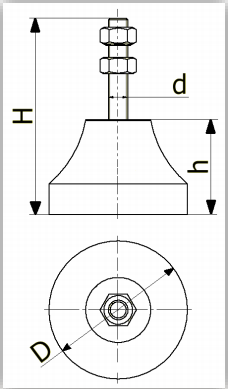
\includegraphics[scale=0.5]{figuras/amortecedor.png}
      \caption{Desenho técnico do pé da bancada. Fonte: \cite{mola_catalogo}}
      \label{fig:pe_bancada}
      \end{figure}


\subsubsection*{\textbf{Faixas de Atuação}}
A faixa de frequência que a mesa poderá vibrar será de 50 a 100 Hz que equivalem a 3000 a 6000 vibrações por minutos. Essa faixa foi escolhida por ser utilizada em mesas vibratórias comerciais \cite{ricardo_jose}.

\subsection*{\textbf{Geometria da mesa}}

	A mesa de vibração terá uma altura de 900mm e dimensões de 500 x 800mm. Com base nestas características e verificando que se trata de uma mesa com geometria retangular foi elaborado um design estrutural da mesa contendo quatro hastes de cantoneira na vertical com reforços frontais e laterais nas alturas de 350mm e 250mm respectivamente. Tais reforços impedirão com que a estrutura da mesa sofra flexão e torção, além disso, servirá de sustentação para fixação do motor. Uma união das hastes verticais será reforçada através de cantoneiras na parte superior da estrutura, reforçando ainda mais as fixações anti-flambagem da mesa, além de servir de apoio para fixação das molas. 
    
    Opções de geometria do tipo treliça foram excluídas por não ser de uso convencional para este tipo de aplicação de mesa, além de verificar uma redução do peso da estrutura não haveria apoio para fixação do motor. Considerando que uma base de estrutura pesada é necessária para que não haja transferência de vibração do motor para esta. A Figura \ref{fig:base_bancada} representa um esboço do design estrutural da base projetado no software SOLIDWORKS\footnote{http://www.solidworks.com/}.

\begin{figure}[!ht]
\centering
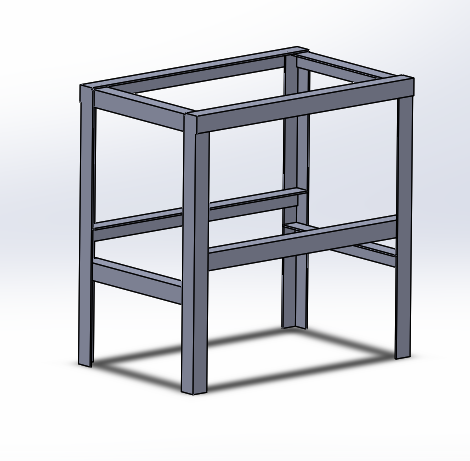
\includegraphics[scale=0.5]{figuras/base_bancada.png}
\caption{Esboço da base da bancada. Fonte: Autores}
\label{fig:base_bancada}
\end{figure}

\subsubsection*{\textbf{Análise modal}}	

Um dos pontos mais importantes da construção de um sistema de vibração mecânica é a região de apoio dos corpos a seres estudados. No caso de uma mesa vibratória é o superfície do tampo. Ele deve ser modelado e construído de forma que permita que a frequência de vibração que foi solicitada de fato seja a que esteja ocorrendo na base do corpo, ou seja, no tampo da mesa.

	Uma análise foi feita nesse sentido para gerar um primeiro parâmetro de escolha do material e da geometria do tampo da mesa. Dentre as decisões de projeto que foram feitas estaca a que a geometria da mesa atenderia alguns requisito de mercado. Um deles era que a superfície da mesas possuísse geometria de 800mm de comprimento por 500mm de profundidade gerando uma área útil de 40000 \[mm^2\], compatível com concorrentes já existentes. Com isso restou apenas uma última variável a ser decidida, a espessura do tampo.
    
	A decisão do tamanho dessa espessura levou em conta duas questões, também decisões de projeto: faixa de vibração entre 50Hz e 100Hz e uso de materiais metálicos para o tampo. Com isso em mente foram feitas análises modais no software de análises Ansys\footnote{www.ansys.com/}, levando em consideração o valor do primeiro modo de vibração. Esse deveria ser, no mínimo, maior que a frequência máxima proposta pela faixa, 100Hz.
    
	A análise modal experimental (AME) consiste em extrair os chamados parâmetros modais de um sistema mecânico. Os parâmetros modais são parâmetros característicos do sistema e são compostos por frequências naturais, fatores de amortecimento e modos de vibrar. Se forem corretamente obtidos é possível descrever o comportamento de um sistema vibratório sem necessitar de um modelo matemático \cite{evandro}.
    
	Uma análise modal inicial leva em conta somente características físicas do material; rigidez e massa. O que pode ser feito tendo como base a biblioteca de materiais do próprio software. 
    
	Na simulação a seguir foram feitos dois ensaios com aço estrutural com espessuras diferentes: 5mm e 10mm. E observou-se o valor do primeiro modo de vibração. O aço estrutural conhecido pelo Ansys se compara ao aço comercial SAE 1010 repuxado a frio (CD). Suas características são apresentadas na Tabela \ref{tab:caracteristicas_aco}.

\begin{table}[!h]
\centering
\caption{Características físicas do aço SAE 1010. Fonte: \cite{shigley}}
\label{tab:caracteristicas_aco}
\begin{tabular}{|l|l|l|l|}
\hline
\multicolumn{1}{|c|}{\textbf{Nº SAE}} & \multicolumn{1}{c|}{\textbf{Processamento}} & \multicolumn{1}{c|}{\textbf{Resistência a tração (Mpa)}} & \multicolumn{1}{c|}{\textbf{Redução de área (\%)}} \\ \hline
1010                                  & CD                                          & 320                                                      & 50                                                 \\ \hline
\end{tabular}
\end{table}

As imagens do teste são apresentadas nas Figuras \ref{fig:analise_1} e \ref{fig:analise_2}. A Figura \ref{fig:analise_1} é relativa ao teste com espessura de 5mm e a Figura \ref{fig:analise_2} com espessura de 10mm. Foi requerido do programa que revolvesse o seis primeiros modos de vibração. Foi somente observado o primeiro. Este deveria ser maior que 100Hz pra evitar ressonância em toda a faixa de uso do equipamento.

\begin{figure}[!ht]
\centering
% 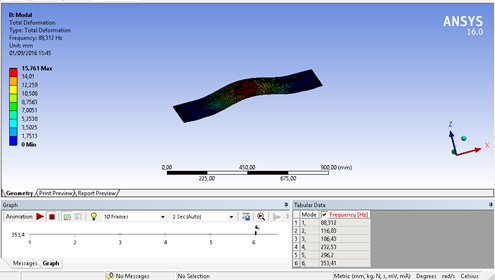
\includegraphics[scale=0.5]{figuras/analise_1.png}
\caption{Ensaio com aço estrutural de 5mm de espessura}
\label{fig:analise_1}
\end{figure}

\begin{figure}[!ht]
\centering
% 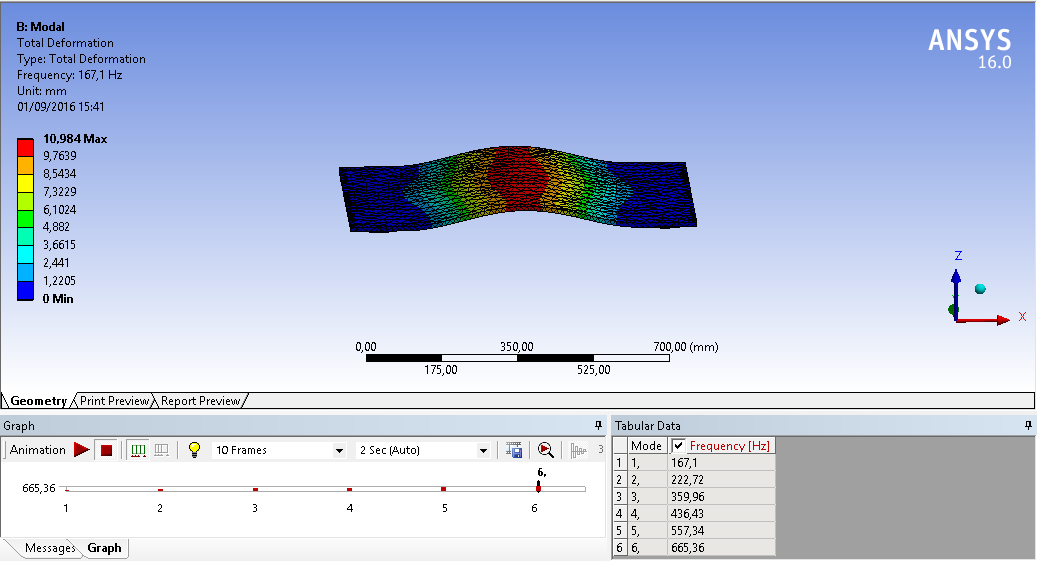
\includegraphics[scale=0.5]{figuras/analise_2.png}
\caption{Ensaio com aço estrutural de 10mm de espessura}
\label{fig:analise_2}
\end{figure}

Dos testes realizados foi observado que a segunda espessura é a indicada pois oferece segurança em toda a faixa de uso; de 50Hz até 100Hz. Pois o primeiro modo de vibração está seguramente acima da frequência máxima. Com um fator de segurança de:

    \begin{equation}
            n = 100 Hz/167,1 Hz = 0,6 
    \end{equation}

Ainda baixo porém já observa-se uma linearidade entre o comprimento da espessura e o valor do primeiro modo de viação.
